\section{Analisi dei dati e classificatori utilizzati}

In questa sezione verrà riportato lo studio effettuato sul dataset.
% Ogni sottosezione tratterà di uno specifico classificatore, dei suoi risultati e degli esperimenti fatti per migliorarne il modello.

\subsection{Considerazioni sugli attributi}

Studiando la composizione dei dati per selezionare le principali tecniche da applicare,
la prima cosa che risulta visibile all'apertura del dataset è sicuramente il suo sbilanciamento nelle classi di output:
come mostrato in~\Cref{fig:classes}, su 100 pazienti in esame, solo 12 risultano compromessi.

\begin{figure}[H]
  \centering
  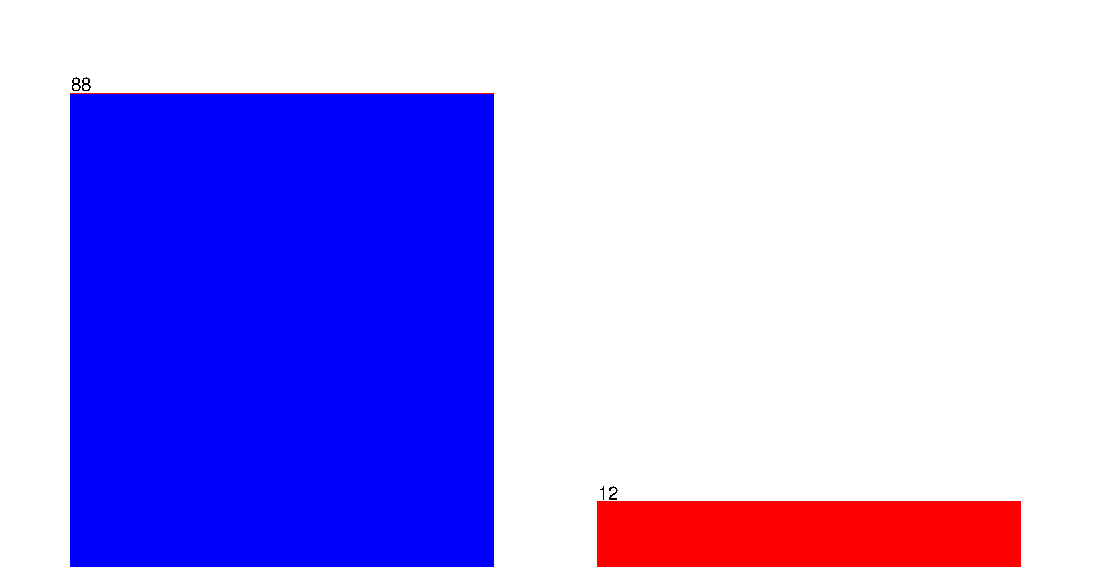
\includegraphics[width=0.85\textwidth]{fig/classes.eps}%
  \caption{%
    L'istogramma rappresenta i valori assunti dall'attributo classe:
    la colonna blu rappresenta le diagnosi di fertilità normale,
    quella rossa gli esami che evidenziano potenziali problematiche.
  }%
  \label{fig:classes}
\end{figure}

Questo disequilibrio tra le classi mette in difficoltà i modelli più semplici;
al fine di ottenere risultati validi, si è messo alla prova diverse configurazioni parametriche.

\todo[inline]{Aggiungere maggiori dettagli per ciascun attributo}

\subsection{Misure di performance dei classificatori}

\todo[inline]{Migliorare quanto segue}

Prima di partire con i vari dati, occorre però stabilire i criteri di misura delle performance dei vari classificatori:
a tale scopo ho tenuto conto in primo luogo della Confusion Matrix prodotta da ogni modello, successivamente dei valori di Precision e Recall per le classi in gioco, attribuendo un maggiore peso ai valori relativi alla classe ``O'' rispetto a ``N'' e infine del valore della ROC\@.
Come modalità di test ho scelto di applicare in ogni situazione la K-Fold Cross-Validation piuttosto che lo splitting statico dei dati in Training e Test Set, la motivazione dietro a questa scelta è l'esiguo numero di dati presenti nel dataset a cui si presta meglio una modalità come il K-Fold Cross-Validation,
in quanto pensata appositamente per dataset di piccole dimensioni.

\todo[inline]{Manca qualcosa?}

\subsection{kNN}
\subsection{Decision Tree}
\subsection{Classificatori Bayesiani}
\subsection{Classificatori Lazy}
\subsection{Multi-Classificatori}
\subsubsection{Approccio Cost-Sensitive}
\subsubsection{Approccio Boosting}
\subsection{Rules}
